\chapter{Perspectives et conclusions} 
  \section{Perspectives} 
 
Le solveur que nous avons élaboré peut-être amélioré de bien des manières.

Un des premiers ajouts que l'on peut imaginer est l'intégration de la génération de puzzle à partir d'une image, partie du sujet non traitée faute de temps et de personnes. Cet ajout pourrait permettre par la suite, éventuellement, la création d'un logiciel de jeu Link-Pix, proposant des grilles à résoudre qui ont été générées par le logiciel à partir d'image.

Un ajout plus «~simple~» serait la gestion des images de couleurs. En effet, on peut imaginer ajouter une caractéristique pour chaque case qui serait la couleur. La possibilité de lier deux indices serait ainsi dépendante de cette couleur, réduisant finalement le champ des possibilités. Une réécriture simple du code permettrait d'intégrer cet ajout.
 
  \section{Conclusions} 
   \subsection{Fonctionnement de l’application} 

   \subsubsection{Généralités}

Bien que notre solveur ait résolu les puzzles que nous lui avons proposés, nous n'avons pas la certitude qu'il puisse résoudre tous les puzzles à solution unique. Ainsi, nous construisons les débuts de chemins dont nous sommes certains, mais nous n'analysons pas si d'autres portions de chemins, situées non pas en début mais au milieu, sont sûres.

\begin{figure}[h!]
      \centering
      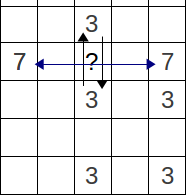
\includegraphics[scale=0.5]{solvable1}
      \caption{On ne peut pas construire de façon sûre les débuts du chemin qui relie les 7, mais il passe forcément entre les deux 3, ce qui peut réduire les possibilités de voisinage.}
\end{figure}

En outre, notre solveur a été testé sur des puzzles de tailles raisonnables, et nous ne pouvons pas savoir avec certitude si les performances sur de plus gros puzzles seront identiques.
Cela dit, le solveur fonctionne sur les problèmes auquels nous l'avons soumis, et il semble efficace tant en utilisation mémoire qu'en temps de calcul.

Ainsi, malgré les problèmes d'organisation que nous avons eu, nous avons atteint notre objectif qui était de fournir un solveur opérationnel, et nous avons même pu créer une interface graphique, alors que nous ne pensions pas en avoir le temps.

\subsubsection{Choix des outils}

Le langage choisi pour développer ce projet, le langage C, aurait sans doute pu être remplacé par un langage de plus haut niveau, ce qui nous aurait permis un développement plus rapide, nous affranchissant ainsi des problèmes de gestion de mémoire. C'était cependant le langage le mieux connu de tous les membres de l'équipe, ce qui nous a permis de travailler plus facilement en groupe.

L'utilisation du gestionnaire de version Git nous a permis de travailler plus facilement à distance, peut-être au détriment de réunions de travail qui auraient pu être plus fréquentes. De même, du retard a été pris suite à certains oublis de soumission, faisant que la version en ligne n'était pas la plus à jour. Il s'est quand même globalement avéré être un outil de choix et a efficacement soutenu notre projet du début à la fin, nous aidant ainsi énormément.

L'utilisation du générateur de documentation Doxygen fut aussi positive. En effet, cet outil s'est avéré facile à utiliser et relativement puissant, nous fournissant ainsi une documentation claire. Nous avions ainsi accès aux caractéristiques d'une fonction beaucoup plus aisément que dans une recherche directement dans le code source.
 
   \subsection{Fonctionnement du groupe de travail} 
 
Les démarrages du projet ont été difficiles, notamment dû au fait que certains membres de l'équipe n'assistaient pas aux réunions. Nous avons ainsi pris du retard au début, les choix ne parvenant pas à être fixés dû aux manques de rigueur des absents.

Cela dit, au milieu du semestre, le retrait complet des étudiants inactifs sur le projet nous a permis de nous mettre au travail en groupe, de façon relativement efficace. Seule une semaine relativement chargée en contrôles nous a fait baisser d'intensité de travail, mais nous avons de façon globale eu un travail assez régulier, jusqu'à la fin où nous avons eu un rythme un peu plus élevé afin d'essayer de terminer dans les temps.

Au final, nous avons réussi à nous entendre, travaillant ensemble et en s'entraidant, de sorte que nous avons pu être relativement efficaces. Les erreurs trouvées étaient rapidement corrigées, notamment grâce à l'utilisation de Git, et nous avons pris du plaisir à travailler ensemble.
